\chapter{Magnetostatics -- Magnetic field resulting from a permanent magnet}

\modinfo{Directory}{Horseshoe}
\modinfo{Solvers}{\Idx{MagnetoDynamics2D}}
\modinfo{Tools}{\Idx{Gmsh}, \Idx{ElmerGUI}}
\modinfo{Dimensions}{2D, Steady-state}
\modinfo{Author}{Peter R{\aa}back}



\subsection*{Case definition}

This case roughly reproduces the case of a permanent magnet as demonstrated in 
the following link: \\
\url{http://www.strek.strefa.pl/students/meslec/lab06.pdf}

Consider a horseshoe-shaped permanent magnet. It consists of a ferromagnetic material but the two end 
sections are premagnetized in opposite directions. This results to a familiar magnetic field pattern.
The horseshoe consists of three different regions and additionally there is the surrounding air.
There is a circular outer boundary in order to conveniently allow for farfield conditions.  
The material is assumed to have a constant relative permeability of 5000 and the magnetization is 
set to 750~kA/m. 

Note that as this is a 2D case the resulting fields actually are those of an infinitely long 
horseshoe which of course does not make much sense in real life. 


\subsection*{Meshing}

The computational mesh is predefined in Gmsh format in file \texttt{horseshoe.msh}. 
If the user wants to modify the default mesh that must be done with Gmsh. The geometry of 
the file is given in file \texttt{horseshoe.geo}.


\subsection*{Solution procedure}

The definitions for the relevant equation are not loaded into ElmerGUI by default. Hence, 
one needs to load these before starting the simulations.
\ttbegin
File 
  Definitions
    Append -> magnetodynamics2d.xml
\ttend
The additional definitions should recide in the directory \texttt{edf-extra} within the distribution.
Moving the desired \texttt{xml} files to the \texttt{edf}-directory enables automatic loading of the 
definitions at start-up. By inspecting the definitions in the \texttt{Elmer Definitions File editor} one
may inspect that the new definitions were really appended. 

The mesh is already defined, load it from the \texttt{samples} directory were it recides.
\ttbegin
File 
  Open -> horseshoe.msh
\ttend
The ElmerGrid plug-in of ElmerGUI will read the mesh and convert it to a format understood by Elmer. 

\begin{figure}[h]
\centering
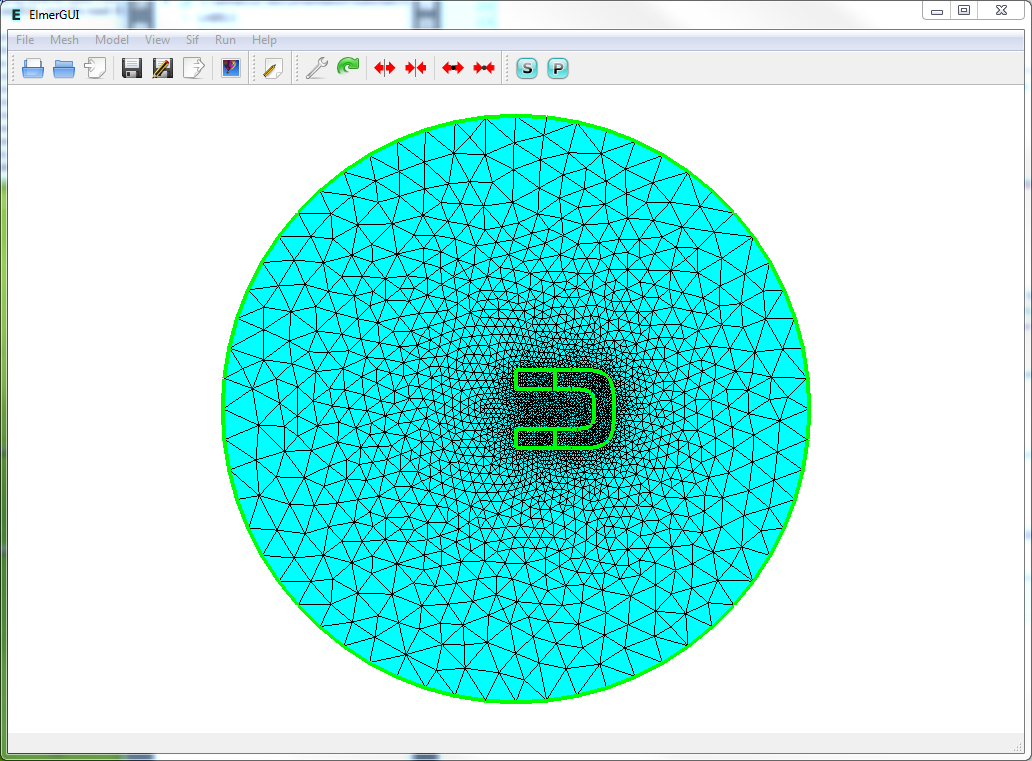
\includegraphics[width=140mm]{HorseShoeMesh}
\caption{The mesh for the horseshoe and surrounding air as see in ElmerGUI}\label{fg:horseshoeselmergui}
\end{figure}  


After we have the mesh we start to go through the Model menu from the top to bottom. 
In the Setup we choose things related to the whole simulation such as file names, 
time stepping, constants etc.
The steady-state simulation is carried out in 2-dimensional cartesian
coordinates. Nothing needs to be changed here. Currently the permeability of vacuum is not given
in the ElmerGUI. To set other than the default value for it, the free text box can be used. 

In the equation section we choose the relevant equations and parameters related to their solution. 
In this case we'll have the MgDyn2D solver, as well as the postprocessing solver MgDyn2DPost.

When defining Equations and Materials it is possible to assign the to bodies immediately, or to use mouse
selection to assign them later. In this case the equations need to be solved in all the bodies and 
hence clicking the all from 1 to 4 here is most convenient. We give a higher priority to the actual solver
so that the vector potential will be computed before the derived fields. 
In this case solver specific options should be ok but they could also be changed in this context.
\ttbegin
Model
  Equation
    Name = MgDyn2D
      Active = on
      Priority = 1
      Apply to Bodies = 1 2 3 4 
    Name = MgDyn2DPost
      Active = on
    Add 
    OK
\ttend        
The Material section includes all the material parameters. In this case we basically have two 
different materials but the differenyt magnetization must also be given as a material property.
Hence we actually need to define four materials.  
\ttbegin
Model
  Material
    Name = Air
    MgDyn2d
      Relative Permeability = 1.0
    Add
    New

    Name = Iron
    MgDyn2d
      Relative Permeability = 5000.0
    Add
    New

    Name = IronPlus
    MgDyn2d
      Relative Permeability = 5000.0
      Magnetization 1 = Real 750.0e3
    Add
    New

    Name = IronMinus
    MgDyn2d
      Relative Permeability = 5000.0
      Magnetization 1 = Real -750.0e3
    Add
    OK
\ttend

We may now assign the material properties by selecting with the mouse.
This spares us of the 
need to know the indexes of each body.
\ttbegin
Model
  Set body properties
    Choose air -> set Materail to Air
    Choose curved part of horseshoe -> set Material to Iron
    Choose upper straight part of horseshoe -> set Material to IronPlus
    Choose lower straight part of horseshoe -> set Material to IronMinus
\ttend

We have just one boundary condition i.e. the outer boundary for which we use the farfield condition.
\ttbegin
Model
  BoundaryCondition
    Name = Farfield
    MgDyn2D
      Infinity BC = True
    Add
    OK
\ttend   

The conditions may also be assigned to boundaries in the Boundary condition menu, or 
by clicking with the mouse. Here we use the latter approach as that spares us of the 
need to know the indexes of each boundary.
\ttbegin
Model
  Set boundary properties
    Choose the 4 pieces of the outer sphere -> set boundary condition Farfield
\ttend

For the execution 
ElmerSolver needs the mesh files and the command file. We have now basically defined
all the information for ElmerGUI to write the command file. After writing it we may also visually 
inspect the command file.
\ttbegin
Sif 
  Generate
  Edit -> look how your command file came out  
\ttend

Before we can execute the solver we should save the files in a directory. The project includes
all the files needed to restart the case.
\ttbegin
File 
  Save Project
\ttend

After we have successfully saved the files we may start the solver
\ttbegin
Run
  Start solver
\ttend
A convergence view automatically pops up showing relative changes of each iteration.
The equation is fully linear and hence only two iterations are needed -- the second 
one just ensures that convergence of the nonlinear level was really obtained. 
The norm of the solution should be 0.3679.

When the solution has finished we may start the postprocessor to view some results.
\ttbegin
Run
  Start ParaView
\ttend


\subsection*{Results}


\begin{figure}[h]
\centering
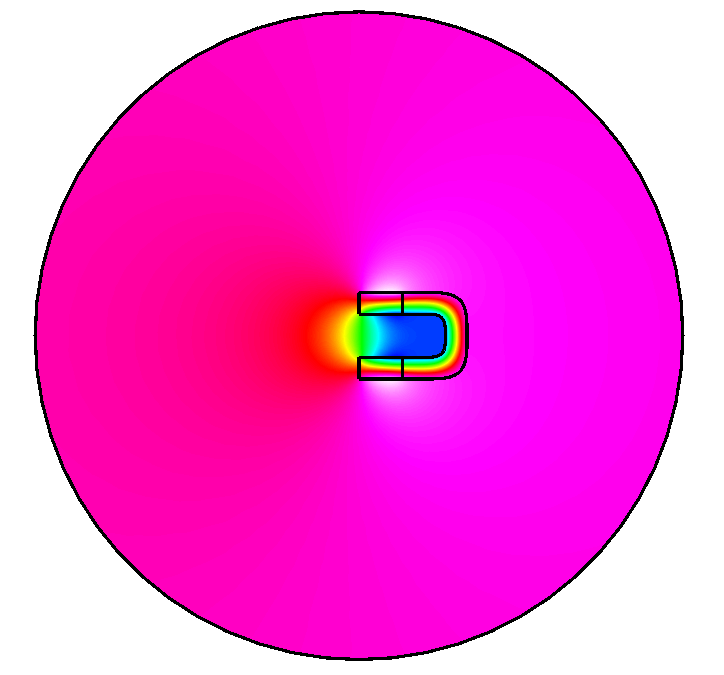
\includegraphics[width=120 mm]{HorseShoeA}
\caption{The vector potential of the magnetic field.}\label{fg:HorseShoeA}
\end{figure}  

\begin{figure}[h]
\centering
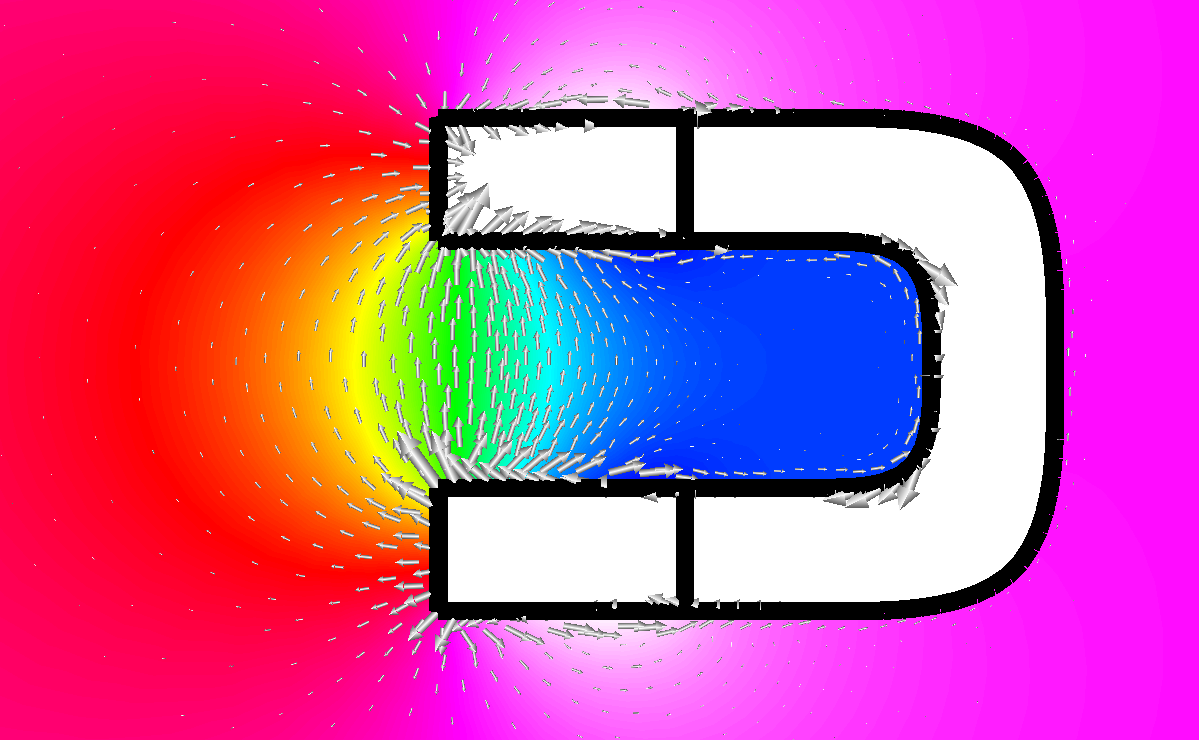
\includegraphics[width=120 mm]{HorseShoeB}
\caption{A closeup of the vector potential combined with the magnetic field intensity vectors. 
Note that the fields in the horseshoe itself have been
masked away to demonstrate the well known field shape in the free space.}\label{fg:HorseShoeB}
\end{figure}  


The resulting z-component of the vector potential is depicted in Figure~\ref{fg:HorseShoeA}.
The corresponding postprocessed magnetic field intensity is depicted in Figure~\ref{fg:HorseShoeB}. 
Note that the derived fields is enforced to be continuous by default which is not 
optimal for visualization. For optimal results use Discontinous Galerkin (DG) method
for the postprocessing. Note that when using DG the postprocessing should be done with .vtu files and 
Paraview. The postprocessing tools of Elmer cannot deal with elementwise-fields. 


\hfill

\bibliography{tutorialsbib}
\bibliographystyle{plain}
